\documentclass[11pt,oneside]{scrbook}
\usepackage[a4paper,margin=2.4cm,marginparwidth=1.8cm,marginparsep=0.4cm]{geometry}
\usepackage{../common/rlstudy}
\usepackage[ruled,vlined,linesnumbered]{algorithm2e}

\title{{\color{rlblue}\textbf{Week 01} \\ \Huge Markov Decision Processes and Bandits}}
\author{STUDY-RL --- a self-paced Deep RL curriculum}
\date{\today}

\begin{document}
\maketitle
\tableofcontents
\newpage

% =============================================================================
\chapter*{Learning objectives}
\addcontentsline{toc}{chapter}{Learning objectives}


% Teaching companion: a small example before the full lecture.
\noindent\textbf{Study companion.} Read \texttt{teaching\_guide.md} in this
folder for step-by-step examples, an analogy with its limits, and self-checks.
Then use \texttt{workbook.ipynb} to implement and vary the calculations.
\par\medskip

\begin{keyidea}
By the end of this week you will be able to:
\begin{enumerate}\setlength\itemsep{2pt}
  \item State the \emph{Markov decision process} tuple $(\States,\Actions,\Tr,R,\Disc)$
        precisely and explain when each component is observable.
  \item Define the multi-armed bandit problem, derive the regret decomposition, and explain the logarithmic horizon
        dependence of the Lai--Robbins lower bound and the UCB1 upper bound.
  \item Implement \texttt{epsilon-greedy}, UCB1, Thompson sampling, and
        Boltzmann/softmax exploration in NumPy and distinguish confidence-based
        optimism, posterior sampling, and action randomisation.
  \item Generalise from MAB to the contextual bandit via \textbf{LinUCB} and
        relate it to off-policy evaluation in the synthetic insurance lead-broker matcher.
  \item Distinguish \emph{discounted} from \emph{average-reward} objectives and
        compute the discounted return $\Ret_t$ for a finite trajectory by hand.
  \item Articulate \emph{why exploration is a safety problem} in any
        high-stakes deployment.
\end{enumerate}
\end{keyidea}

% =============================================================================
\chapter{Motivation \& intuition}
\label{ch:motivation}

\marginnote{The \emph{environment} is the part of the world the agent cannot
inspect, only probe.}%
Reinforcement learning is the study of \emph{agents that learn by doing}. An
agent receives observations from an environment, picks an action, gets a scalar
reward, and the loop repeats. The agent's goal is to maximise the total reward
it accumulates over time. Three ingredients distinguish RL from supervised
learning:

\begin{enumerate}\setlength\itemsep{2pt}
  \item \emph{Feedback is evaluative, not instructive.} The environment tells
        the agent how good its choice was, not which choice was best.
  \item \emph{Decisions compound.} Today's action changes tomorrow's state, so
        the loss surface is non-stationary in a structured way.
  \item \emph{Behaviour shapes the data.} Data may be collected by the current
        policy (on-policy), another policy (off-policy), or a fixed historical
        logger (offline). The data distribution and the learning target must
        therefore be distinguished.
\end{enumerate}

\begin{intuition}
If supervised learning is ``here is the right answer, copy it'', RL is
``commit to an answer, find out later, and don't poison the next ten questions
while you are figuring it out''.
\end{intuition}

\paragraph{From an ML/DL background.} If you have trained a neural net on
\textsc{ImageNet}, you have already seen the easy half of RL: function
approximation. The hard half is the \emph{data-generation loop}. In RL you
choose the dataset as you go --- and choosing it badly is what causes most
real-world failures, not bad gradients.

\paragraph{Bandits first.} Before we bring in transitions, we strip the
problem of state and look at the \emph{multi-armed bandit (MAB)}: $K$ slot
machines, each with an unknown reward distribution; pick one per round; how
fast can you discover the best? Bandits provide a useful starting model for
matching decisions. ``Which broker should I show this lead to?'' can be
modelled as a contextual bandit; choosing an ordered shortlist can be
modelled as a slate bandit. Whether a real matcher is well
modelled as a bandit depends on delayed outcomes, capacity constraints,
interference, and whether current decisions change future opportunities.

\begin{figure}[h]\centering
\begin{tikzpicture}[->,>={Stealth},thick,node distance=2.6cm,
  agent/.style={rectangle,rounded corners=2pt,fill=rlblue!10,
                draw=rlblue,minimum height=10mm,minimum width=22mm,font=\sffamily},
  env/.style={rectangle,rounded corners=2pt,fill=rlteal!10,
              draw=rlteal,minimum height=10mm,minimum width=22mm,font=\sffamily}]
  \node[agent] (A) {Agent $\Policy$};
  \node[env, right=of A] (E) {Environment $\Tr,R$};
  \draw[->] (A.north east) to[bend left=20] node[above]{$a_t$} (E.north west);
  \draw[->] (E.south west) to[bend left=20]
        node[below]{$(s_{t+1}, r_{t+1})$} (A.south east);
\end{tikzpicture}
\caption{The agent--environment loop. Bandits are the special case where the
state never changes, so the only choice is the action.}
\label{fig:loop}
\end{figure}

\begin{pitfall}
\textbf{Reward is not a loss.} A negative reward is a \emph{penalty}, not a
signal that you should ``learn less''. Beginners flip the sign of the reward
when porting supervised code, train a policy that minimises return, and
conclude that ``RL doesn't work''. Always check the sign convention before
debugging anything else.
\end{pitfall}

% =============================================================================
\chapter{Mathematical formulation}
\label{ch:math}

\section{Multi-armed bandits}

\begin{definition}[Stochastic multi-armed bandit]
A \emph{stochastic $K$-armed bandit} is a tuple $(\Actions,\, \{\nu_a\}_{a\in\Actions})$
where $\Actions=\{1,\dots,K\}$ is the set of arms and each $\nu_a$ is a
probability distribution over $\mathbb{R}$ with mean
$\mu_a = \E_{R\sim\nu_a}[R]$. At each round $t = 1,2,\dots$ the learner
selects $A_t\in\Actions$ and observes a fresh reward from $\nu_{A_t}$,
conditionally independent of the past given the selected arm.
\end{definition}

Let $\mu^\star = \max_a \mu_a$ and $\Delta_a = \mu^\star - \mu_a \ge 0$. The
\emph{cumulative regret} after $T$ rounds is
\begin{equation}
R_T \defeq T\mu^\star - \E\!\left[\sum_{t=1}^T R_t\right]
     = \sum_{a=1}^K \Delta_a \E[N_a(T)],
\label{eq:regret-decomp}
\end{equation}
where $N_a(T) = \sum_{t=1}^T \mathbf{1}\{A_t=a\}$. The decomposition on the
right is the foundation of every regret proof in this lecture: \emph{regret is
the total time spent on sub-optimal arms, weighted by how sub-optimal each is}.

\begin{theorem}[Lai--Robbins lower bound, 1985]
For a uniformly efficient algorithm (expected regret $o(T^c)$ for every
$c>0$ on every Bernoulli instance), with means in $(0,1)$ and any
suboptimal arm $a$,
\[
\liminf_{T\to\infty} \frac{\E[N_a(T)]}{\log T} \ge \frac{1}{\KL(\nu_a, \nu^\star)},
\]
hence $R_T \ge (1+o(1))\sum_{a:\Delta_a>0}\frac{\Delta_a}{\KL(\nu_a,\nu^\star)}\log T$.
\end{theorem}

\begin{proof}[Sketch]
Change-of-measure argument. If the algorithm rarely pulled $a$ under the true
problem, it could not distinguish it from a perturbed problem where $a$ has
mean $\mu^\star + \epsilon$, with perturbed reward law $\nu'_a$. The KL
between the two interaction-history laws is
$\E[N_a(T)]\KL(\nu_a,\nu'_a)$ because only this arm's reward law changes.
Uniform efficiency forces this information to grow at least as
$(1-o(1))\log T$. Taking $\epsilon$ down to zero yields the Bernoulli
denominator in the theorem. \qedhere
\end{proof}

\begin{theorem}[UCB1, Auer--Cesa-Bianchi--Fischer 2002]
Suppose stationary independent arm rewards lie in $[0,1]$ almost surely,
and pull every arm once initially. The UCB1 policy
\[
A_{t+1} = \argmax_a \;\hat\mu_a(t) + \sqrt{\frac{2\log t}{N_a(t)}}
\]
satisfies
\begin{equation}
R_T \;\le\; \sum_{a:\Delta_a>0}\frac{8\log T}{\Delta_a}
         \;+\; \Big(1+\tfrac{\pi^2}{3}\Big)\sum_{a:\Delta_a>0}\Delta_a.
\label{eq:ucb1-bound}
\end{equation}
\end{theorem}

\begin{proof}[Sketch with explicit count union]
Fix a suboptimal arm $a$ and horizon $T\ge K$. Let
$\ell=\lceil8\log T/\Delta_a^2\rceil$ and $c_{t,n}=\sqrt{2\log t/n}$.
After $t$ total pulls, the two sample counts are adaptive. For fixed counts
$n_*,n_a\le t$, Hoeffding bounds each of the one-sided bad events
\[
\hat\mu_{*,n_*}\le\mu^*-c_{t,n_*},\qquad
\hat\mu_{a,n_a}\ge\mu_a+c_{t,n_a}
\]
by $t^{-4}$. If neither occurs and $n_a\ge\ell$, then the optimal arm's
index is strictly above $\mu^*$, while arm $a$'s index is strictly below
$\mu_a+2c_{t,n_a}\le\mu^*$, so arm $a$ cannot be selected.
Union-bound over both possible counts, not just the suboptimal arm's count:
\[
\Prb\{A_{t+1}=a,N_a(t)\ge\ell\}
\le \sum_{n_*=1}^{t}\sum_{n_a=\ell}^{t}2t^{-4}
\le2t^{-2}.
\]
There are at most $\ell$ pulls before the threshold. Hence
$\E[N_a(T)]\le8\log T/\Delta_a^2+1+\pi^2/3$.
Multiply by each gap and sum to obtain~\eqref{eq:ucb1-bound}.
\end{proof}

\begin{remark}
Compare like quantities: the regret coefficients are $8/\Delta_a$ and
$\Delta_a/\KL(\nu_a,\nu^*)$, whereas the pull-count coefficients are
$8/\Delta_a^2$ and $1/\KL(\nu_a,\nu^*)$.
For fixed interior Bernoulli mean $q=\mu^*\in(0,1)$ and small gap,
$\KL(\mathrm{Bern}(q-\Delta),\mathrm{Bern}(q))
=\Delta^2/[2q(1-q)]+O(\Delta^3)$.
Thus both regret coefficients scale as $1/\Delta$ in this regime, with
different constants. This is not a uniform constant-factor statement as
means approach the boundaries. KL-UCB can attain the Bernoulli asymptotic
lower-bound coefficient under its stated assumptions.
\end{remark}

\begin{theorem}[Thompson sampling for Bernoulli arms, Agrawal--Goyal 2012]
\label{thm:ts}
With Beta(1,1) priors and posterior update $\alpha_a\gets\alpha_a+R_t$,
$\beta_a\gets\beta_a+1-R_t$ after observing arm $a$, the Thompson policy
$A_{t+1}=\argmax_a \tilde\mu_a$ where $\tilde\mu_a\sim\mathrm{Beta}(\alpha_a,\beta_a)$
achieves
\[
R_T \le O\!\left(\sum_{a:\Delta_a>0}\frac{\log T}{\Delta_a}\right).
\]
\end{theorem}

\begin{proof}[Idea]
At each round the posterior concentration around the true means happens at the
Bernstein rate. The probability that a suboptimal posterior beats the optimal
posterior is bounded by an integral over the gap in beta-CDFs, which is
$O(1/t^{1+\epsilon})$ once $N_a(t)\ge \tfrac{c\log t}{\Delta_a^2}$. Russo--Van
Roy's \emph{information ratio} argument gives the cleanest unified proof.
\qedhere
\end{proof}

\paragraph{Boltzmann / softmax exploration.}
$\Prb(A_t=a) = \exp(\hat\mu_a/\tau) / \sum_b \exp(\hat\mu_b/\tau)$. Temperature
$\tau\to 0$ recovers the greedy policy; $\tau\to\infty$ uniformises. Boltzmann
exploration has no $\log T$ regret guarantee in general because it can stop
exploring sub-optimal arms whose estimates are far below the optimum, even when
the estimates are very uncertain. It is, however, ubiquitous in deep RL
(\textsc{soft actor-critic} uses an entropy-regularised analogue).

\section{Contextual bandits and LinUCB}

\begin{definition}[Stochastic contextual bandit]
At round $t$ the learner observes a context $X_t\in\Real^d$ drawn i.i.d.\ from
an unknown distribution, selects $A_t\in\Actions$, and observes
$R_t = \langle X_t, \theta^\star_{A_t}\rangle + \eta_t$ where
$\eta_t$ is $\sigma$-sub-Gaussian conditional on the past, and the
$\theta^\star_a\in\Real^d$ are unknown. \emph{Linear} bandits have a single
shared $\theta^\star$; the disjoint-arm variant has one per arm.
\end{definition}

LinUCB maintains, per arm,
\[
A_a^{(t)} = \lambda I + \sum_{s\le t : A_s = a} X_s X_s^\top,
\quad
b_a^{(t)} = \sum_{s\le t : A_s = a} R_s X_s,
\quad
\hat\theta_a^{(t)} = (A_a^{(t)})^{-1} b_a^{(t)},
\]
and acts by
\begin{equation}
A_{t+1} = \argmax_a \;\langle X_{t+1}, \hat\theta_a^{(t)}\rangle
         + \alpha\sqrt{X_{t+1}^\top (A_a^{(t)})^{-1} X_{t+1}}.
\label{eq:linucb}
\end{equation}
The bonus is the radius of the elliptical confidence region for $\theta^\star_a$,
projected onto the current context. Abbasi-Yadkori, Pál \& Szepesvári (2011)
prove a problem-independent $\tilde O(d\sqrt{T})$ regret bound for the
single-$\theta^\star$ case under self-normalised concentration.

\section{Markov decision processes}

\begin{definition}[Finite MDP]
A finite Markov decision process is a tuple
$\mathcal{M}=(\States,\Actions,\Tr,R,\Disc)$:
\begin{itemize}\setlength\itemsep{1pt}
  \item $\States$ a finite state space; $\Actions$ a finite action space.
  \item $\Tr: \States\times\Actions \to \Delta(\States)$ the transition kernel,
        $\Tr(s'\mid s,a)$.
  \item $R: \States\times\Actions\times\States \to \Real$ the conditional
        mean reward function. A joint kernel $p(s',r\mid s,a)$ describes
        stochastic rewards; assume sampled rewards satisfy $|r|\le R_{\max}$.
  \item $\Disc\in[0,1)$ the discount factor (for episodic MDPs we allow
        $\Disc=1$ when the return is integrable, for example with bounded
        rewards and finite expected episode length under the policies considered).
\end{itemize}
The \emph{Markov property} is the statement that, given $S_t$ and $A_t$, the
random variables $(S_{t+1}, R_{t+1})$ are independent of all earlier history.
\end{definition}

\begin{definition}[Return]
For a trajectory $(S_0,A_0,R_1,S_1,A_1,R_2,\dots)$, the \emph{discounted return}
is $\Ret_t \defeq \sum_{k=0}^{\infty} \Disc^k R_{t+k+1}$.
\end{definition}

\paragraph{Discounted vs.\ average reward.} Two scalar criteria coexist in the
literature:
\begin{itemize}\setlength\itemsep{1pt}
  \item \emph{Discounted}: $J_\gamma(\Policy)=\E_\Policy[\sum_{t\ge 0}\Disc^t R_{t+1}]$. Algorithms enjoy
        contraction at rate $\Disc$ (Week 2) but the answer depends on the
        somewhat arbitrary choice of $\Disc$.
  \item \emph{Average reward}: $J_{\mathrm{avg}}(\Policy)=\lim_{T\to\infty}\tfrac{1}{T}\E_\Policy[\sum_{t=1}^T R_t]$.
        Independent of an arbitrary discount and is the right criterion for
        long-running matching marketplaces, but the Bellman equation involves a
        \emph{differential} value $h(s)$ and the bias-optimality theory is more
        delicate (Puterman 1994, Ch.\ 8).
\end{itemize}
For synthetic insurance, where the time horizon between a lead arriving and a policy bind
is days to weeks, $\Disc\in[0.95, 0.99]$ at a daily step gives sensible
behaviour; for ATS, with weeks-to-hire, $\Disc\approx 0.99$ at a weekly step.

\begin{pitfall}
\textbf{Don't confuse $\gamma$ with a regulariser.} Lowering $\gamma$ does not
make learning ``easier'' --- it changes the objective. A myopic agent
(\(\gamma\)$\to 0$) is solving a different problem from a far-sighted agent and
will pick different actions in non-trivial MDPs.
\end{pitfall}

% =============================================================================
\chapter{Algorithms}
\label{ch:algos}

\begin{algorithm}[H]
\SetAlgoLined
\KwIn{horizon $T$, exploration parameter $\epsilon$.}
Initialise $\hat\mu_a\gets 0$, $N_a\gets 0$ for all $a$.\;
\For{$t=1,\dots,T$}{
  With probability $\epsilon$, pick $A_t$ uniformly at random\;
  Otherwise $A_t \gets \argmax_a \hat\mu_a$\;
  Observe $R_t\sim\nu_{A_t}$; update $N_{A_t}\!\mathrel{+}=\!1$,
  $\hat\mu_{A_t}\mathrel{+}=\!\tfrac{1}{N_{A_t}}(R_t-\hat\mu_{A_t})$\;
}
\caption{$\epsilon$-greedy bandit.}
\end{algorithm}

\begin{algorithm}[H]
\SetAlgoLined
\KwIn{horizon $T$, exploration constant $c=2$.}
Pull each arm once to initialise; then for $t=K+1,\dots,T$:\;
$A_t \gets \argmax_a \hat\mu_a + \sqrt{c\log t / N_a}$\;
Observe $R_t$; update $\hat\mu_a$, $N_a$ incrementally as above.\;
\caption{UCB1.}
\end{algorithm}

\begin{algorithm}[H]
\SetAlgoLined
\KwIn{Beta$(1,1)$ priors $\{\alpha_a,\beta_a\}$.}
\For{$t=1,\dots,T$}{
  Sample $\tilde\mu_a\sim\mathrm{Beta}(\alpha_a,\beta_a)$ for each $a$\;
  $A_t\gets \argmax_a \tilde\mu_a$\;
  Observe $R_t\in\{0,1\}$; $\alpha_{A_t}\mathrel{+}=R_t$, $\beta_{A_t}\mathrel{+}=1-R_t$\;
}
\caption{Beta-Bernoulli Thompson sampling.}
\end{algorithm}

\begin{algorithm}[H]
\SetAlgoLined
\KwIn{ridge $\lambda>0$, bonus $\alpha>0$.}
For each arm $a$: $A_a\gets\lambda I_d$, $b_a\gets 0$.\;
\For{$t=1,\dots,T$}{
  Observe context $X_t$\;
  For each $a$: $\hat\theta_a\gets A_a^{-1}b_a$;
  $u_a\gets X_t^\top\hat\theta_a + \alpha\sqrt{X_t^\top A_a^{-1} X_t}$\;
  $A_t\gets\argmax_a u_a$; observe $R_t$\;
  $A_{A_t}\mathrel{+}= X_t X_t^\top$;\quad $b_{A_t}\mathrel{+}= R_t X_t$\;
}
\caption{LinUCB (disjoint arms).}
\end{algorithm}

\begin{example}[Worked update]
Suppose two Bernoulli arms with current Beta posteriors
$(\alpha_1,\beta_1) = (3,2)$ and $(\alpha_2,\beta_2)=(1,4)$. A single Thompson
sample might return $\tilde\mu_1=0.62$ and $\tilde\mu_2=0.15$, so the agent pulls
arm 1. If the reward is $R_t=0$, the posterior becomes
$(\alpha_1,\beta_1)=(3,3)$. Its mean falls from $0.6$ to $0.5$, while
its variance falls from $0.04$ to $1/28\approx0.0357$. A disappointing
observation need not increase posterior uncertainty.
\end{example}

\paragraph{Complexity.} Per-round cost is $O(K)$ for $\epsilon$-greedy/UCB1/TS;
$O(K d^2)$ for LinUCB because of the $A_a^{-1}$ multiplication (Sherman--Morrison
brings the matrix update to $O(d^2)$).

\begin{pitfall}
\textbf{Logarithm-of-zero.} UCB1 must be initialised by pulling each arm at
least once, otherwise the $\sqrt{2\log t/N_a}$ bonus is infinite or undefined
and the first $K$ rounds are determined by floating-point quirks.
\end{pitfall}

% =============================================================================
\chapter{Implementation walkthrough}

The mini-project lives in \texttt{project/}. The agents are
deliberately written as small dataclasses so you can inspect their internal
state in the notebook.

\begin{codebox}
\begin{minted}{python}
# project/agent.py (excerpt)
@dataclass
class UCB1Agent:
    K: int; c: float = 2.0; seed: int = 0
    def __post_init__(self):
        self.rng = np.random.default_rng(self.seed)
        self.counts = np.zeros(self.K, dtype=int)
        self.means  = np.zeros(self.K, dtype=float)
    def select(self, t):
        unplayed = np.flatnonzero(self.counts == 0)
        if unplayed.size:
            return int(unplayed[0])
        bonuses = np.sqrt(self.c * np.log(max(t, 2)) / self.counts)
        ucb = self.means + bonuses
        return int(self.rng.choice(np.flatnonzero(ucb == ucb.max())))
    def update(self, a, r):
        self.counts[a] += 1
        self.means[a]  += (r - self.means[a]) / self.counts[a]
\end{minted}
\end{codebox}

The synthetic insurance-style contextual environment (\texttt{project/env.py}) generates a
non-intercept feature vector with $X_{t,j}\sim\mathcal{N}(0,0.7^2)$ (with $X_{t,1}\equiv 1$ as an intercept
slot) and computes the binding probability via a sigmoid of
$\langle X_t,\theta_a^\star\rangle + b_a$. The latent $\theta_a^\star$ matrix is
drawn once per environment construction, using its seed. It is fixed within
that environment; changing the seed changes both the latent instance and
the generated observations. The sigmoid reward means are not exactly linear,
so LinUCB here is an approximation rather than a direct application of its
linear-model regret guarantee.

\paragraph{Reproducibility.} Every agent receives a deterministic seed; the
environment uses an independent generator so reward noise does not co-vary with
agent randomness. This isolates the variance you see in figures to environment
noise plus exploration noise.

% =============================================================================
\chapter{Empirical results}

\begin{figure}[ht]\centering
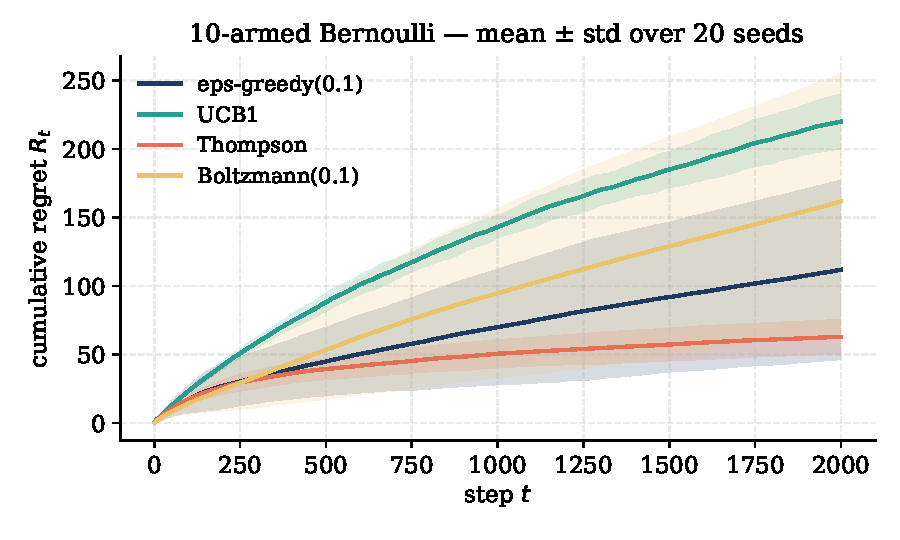
\includegraphics[width=0.92\linewidth]{figs/fig_bernoulli_bakeoff.pdf}
\caption{10-armed Bernoulli testbed. Means $\in[0.1,0.7]$ in steps of $0.05$,
$T=2000$, 20 seeds. Thompson sampling clearly dominates; UCB1 ($c=2$) is
over-exploratory in the first $\sim 500$ rounds but its slope flattens
sub-linearly afterwards. Boltzmann ($\tau=0.1$) is competitive but
hyper-parameter sensitive.}
\label{fig:bakeoff}
\end{figure}

\begin{figure}[ht]\centering
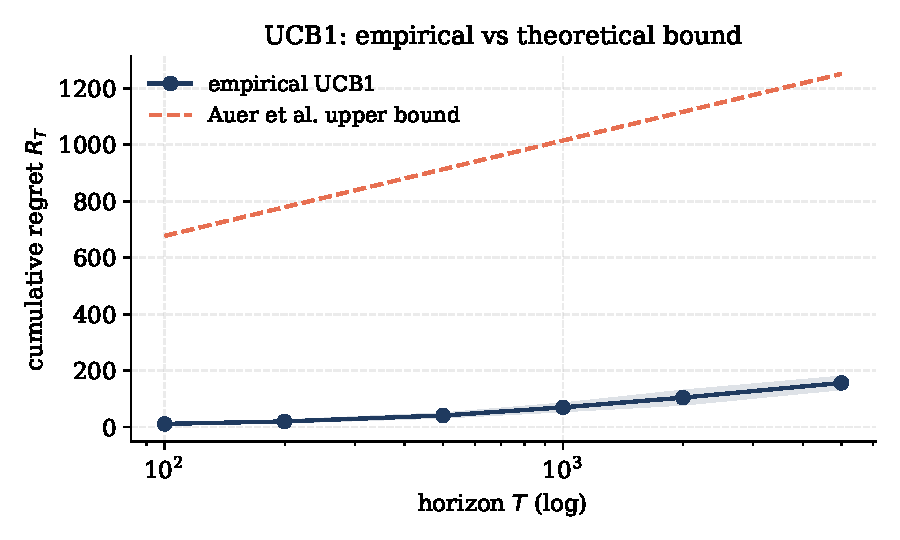
\includegraphics[width=0.92\linewidth]{figs/fig_regret_bound.pdf}
\caption{Empirical UCB1 regret vs the Auer et al.\ theoretical upper
bound~\eqref{eq:ucb1-bound} on a 4-arm Bernoulli with gaps
$\Delta\in\{0.1,0.2,0.3\}$. The empirical curve sits well below the bound,
which is loose by a constant but matches the slope.}
\label{fig:bound}
\end{figure}

\begin{figure}[ht]\centering
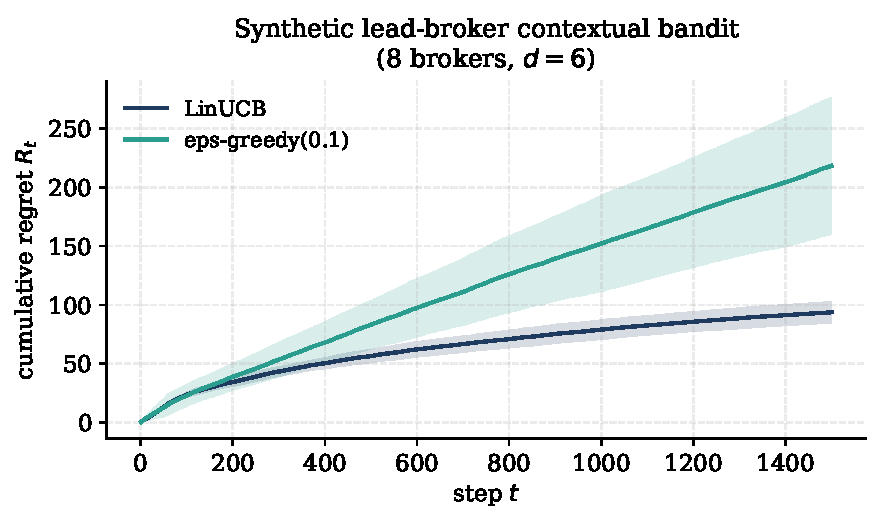
\includegraphics[width=0.92\linewidth]{figs/fig_contextual_bandit.pdf}
\caption{synthetic insurance lead-broker contextual bandit (8 brokers, $d=6$).
LinUCB exploits the context structure and achieves sub-linear regret;
$\epsilon$-greedy ignores the context and grows linearly.}
\label{fig:contextual}
\end{figure}

\begin{intuition}
The slope of regret \emph{after} the burn-in phase is the diagnostic you care
about. A bandit algorithm with steep early regret but a clean log-linear tail
is much safer than one with a flat early curve that turns linear in the long
run --- the latter is silently mis-calibrating its uncertainty.
\end{intuition}

% =============================================================================
\chapter{Safety angle}

\begin{safetyangle}
\textbf{Exploration in a high-stakes domain.}
Pure $\epsilon$-greedy is the most popular reinforcement-learning idea and the
most dangerous one to deploy in matching. Three concrete failure modes:

\begin{enumerate}\setlength\itemsep{2pt}
  \item \emph{Uniform exploration on a sensitive feature.} If your context
        includes a protected attribute (e.g.\ postcode in the UK, which proxies
        for ethnicity), an $\epsilon$-greedy router sprays leads uniformly over
        brokers, including some who are systematically worse on certain
        cohorts. Over a few weeks of logs this looks like demographic-parity
        violation, and you cannot disentangle exploration noise from broker
        bias.
  \item \emph{Unbounded posterior pulls.} Thompson sampling will, with positive
        probability, sample from the tail of a flat posterior and pick a broker
        with no track record. Without a \emph{floor} on the number of
        observations per arm, that one tail sample can route a high-value
        commercial lead to a broker who has never handled commercial. This is
        not a bug in TS --- it is the cost of exploration --- and the right
        response is a domain-specific safety filter, not abandoning TS.
  \item \emph{Mis-specified rewards.} If the operator logs binding as the
        reward but the platform is paid on revenue, you maximise binds and
        leave revenue on the table; worse, you train brokers to bind cheap and
        cancel later, gaming the optimised metric. Reward design is a safety
        problem.
\end{enumerate}

\paragraph{Mitigations.} \textbf{(i)} Cap $\epsilon$-greedy with a
\emph{minimum-traffic gate}: a broker must have $N_a\ge n_{\min}$ before being
eligible for high-value leads, and the first $n_{\min}$ pulls come only from
low-value leads with bounded downside. \textbf{(ii)} Use \emph{shielded
exploration}: a hard rules layer rejects any action a regulator would flag,
applied \emph{after} the bandit chooses (see Alshiekh et al., AAAI
2018; Achiam et al., CPO, ICML 2017). \textbf{(iii)} Log
$\pi_b(a\mid x)$, not just $a$ --- without propensities, every downstream OPE
estimate is biased and you cannot audit anything.

\paragraph{Citations.}
\textsc{Alshiekh, Bloem, Ehlers, K\"onighofer, Niekum, Topcu --- Safe RL via
Shielding, AAAI 2018 (arXiv:1708.08611)};
\textsc{Joachims, Swaminathan, de Rijke --- Deep Learning with Logged Bandit
Feedback, ICLR 2018}.
\end{safetyangle}

% =============================================================================
\chapter{Matching application}

\begin{matching}
\textbf{synthetic insurance lead-broker matcher as a contextual bandit.}
A lead $x\in\Real^d$ encodes postcode hash, vehicle / property descriptors,
prior claim summary, derived text-embedding of the free-text question, and a
constant intercept. Action $a\in\{1,\dots,K\}$ is the broker; reward
$r\in\{0,1\}$ is the binding event observed days later.

\paragraph{When is a bandit sufficient?} The one-step model assumes that
routing choices do not materially change future opportunities. Adding the
current queue to the context helps predict immediate outcomes, but does not
remove the effect of today's action on tomorrow's queue. If those effects
matter to the objective, include them in a sequential model. Delayed feedback
is a separate issue (Chapelle 2014; see Week 11).

\subsection*{Mapping the math}
\begin{tabular}{@{}p{1.3cm}p{\dimexpr\linewidth-1.3cm-2\tabcolsep\relax}@{}}
$X_t$ & lead feature vector at time $t$ \\
$A_t$ & broker chosen by the policy \\
$\theta^\star_a$ & latent ``binding affinity'' of broker $a$ across feature
                   dimensions \\
$R_t$ & 1 if a policy is bound within the SLA window, 0 otherwise \\
$\pi_b$ & current production routing policy (e.g.\ rule-based) \\
$\pi$ & candidate new policy (LinTS / LinUCB)
\end{tabular}

\paragraph{Experiment to run.} Compare LinUCB and $\epsilon$-greedy on the
same synthetic instances, reporting cumulative regret across seeds
(Figure~\ref{fig:contextual}). A synthetic improvement does not establish
an effect size on real routing data, where true regret is generally unobserved.

The ATS equivalent (Week 1 is also relevant to candidate ranking) is the
same bandit with $X_t$ = candidate embedding, $A_t$ = job requisition, $R_t$ =
interview-yes. Position-bias correction (Joachims--Swaminathan--Schnabel 2017)
is one ingredient of the CLTR pipeline studied in Week 12.
\end{matching}

% =============================================================================
\chapter{Exercises}
\label{ch:exercises}

Full versions with hints and graded tests are in \texttt{workbook.ipynb}.
Reference solutions are in \texttt{project/solutions.py}.

\begin{enumerate}[label={},leftmargin=0pt,labelsep=0pt]\setlength\itemsep{2pt}
  \item \textbf{Ex.\ 1 ($\star$).} Implement the incremental sample-average
        update $Q_n = Q_{n-1} + \tfrac{1}{n}(R_n - Q_{n-1})$ and verify it equals
        $\bar R_n$ to floating-point precision.
  \item \textbf{Ex.\ 2 ($\star$).} Run $\epsilon$-greedy on a 3-arm Bernoulli
        with gaps $(0.6,0.3,0.0)$ for $T=200$. Plot cumulative regret. Why is
        it non-decreasing?
  \item \textbf{Ex.\ 3 ($\star\star$).} Implement the UCB1 bonus
        $\sqrt{2\log t/N_a}$. Verify that the bonus shrinks as $N_a\to\infty$
        and is infinite for unpulled arms.
  \item \textbf{Ex.\ 4 ($\star\star$).} Show that after observing
        $s$ successes and $n-s$ failures on a Beta(1,1) prior, the posterior is
        Beta$(1+s,1+n-s)$. Implement the update.
  \item \textbf{Ex.\ 5 ($\star\star$).} Bake off $\epsilon$-greedy vs UCB1 vs
        TS on a 4-arm Bernoulli with $T=500$ and 5 seeds. Tabulate final
        regret. Which algorithm has the lowest variance across seeds?
  \item \textbf{Ex.\ 6 ($\star\star$).} Compute the discounted return of the
        reward sequence $(1, 1, 1)$ for $\gamma=0.5$ by hand, then verify with
        code. Repeat for $\gamma=1$ and the sequence $(0,0,10)$.
  \item \textbf{Ex.\ 7 ($\star\star$).} Run LinUCB and $\epsilon$-greedy on the
        synthetic insurance contextual bandit for $T=1500$. Plot cumulative regret. The gap
        is the value of using context.
  \item \textbf{Ex.\ 8 ($\star\star\star$, open-ended).} Implement the
        \emph{Self-Normalised IPS} (SNIPS) off-policy estimator
        $\widehat V(\pi) = \sum_i w_i r_i / \sum_i w_i$. Use it to estimate
        the value of a candidate policy from logs of a different behaviour
        policy. Discuss when SNIPS is biased vs.\ when it is dangerous.
\end{enumerate}

% =============================================================================
\chapter{Further reading}

The companion document \texttt{extended\_reading.pdf} unpacks five papers in
depth: Robbins (1952), Auer--Cesa-Bianchi--Fischer (2002), Agrawal--Goyal
(2012), Li--Chu--Langford--Schapire (2010), and Russo--Van Roy (2014). The
bandit dossier in \texttt{research/bandits\_matching\_sota.md} is the source
material; this week's reading list is a curated entry point.

\end{document}
